\documentclass[10pt]{article}
\usepackage{icmlko}

\icmlmeta{IP 파운데이션 월드모델}{234}{채운 것과 잰 것을 섞어 적는다}{노트 233이 ``채우면 이기나''를 물었다. 판으로는 안 갈리는데 도메인별로는 크게 갈린다 --- 평균이 반대 방향을 지우는 것을 세 번째로 본다}

\begin{document}

\twocolumn[
\icmlheader

\begin{abstract}
노트 233이 ``하네스가 정직한 정식화를 벌하면 포트폴리오는 대입하는 쪽으로
자란다''를 남기고 \textbf{대입한 것과 관측한 것을 판정치가 구분하는지}를
물었다. 쟀다. 먼저 규모다 --- \textbf{유보 행의 축 관측률 중앙이 도메인마다
0.53$\sim$0.79 라, 모든 행에서 축의 4분의 1에서 절반이 대입값이다.}
관측률 0.7 로 갈라 두 판을 적으니 \textbf{판 전체로는 거의 안 갈린다} ---
F6 능형 $+$0.0125 · F21 $+$0.0092 · F23 $+$0.0116 이고 \textbf{F18 배깅은
$-$0.0081 로 오히려 대입 쪽에서 낫다.} 여기서 멈추면 ``대입이 공짜도
아니고 벌도 아니다''가 된다. \textbf{도메인별로 갈라 보면 다르다} ---
모바일이 \textbf{$+$0.21}(F18 $+$0.217 · F23 $+$0.215), 팝업이
$+$0.11$\sim$0.12, \textbf{애니는 $-$0.05} 다. \textbf{판 $\pm$0.01 은 큰
값들이 서로 지운 결과다.} 그리고 이 모양을 이 사이클에서 세 번째로 본다 ---
노트 225(라벨 성질로 가르니 계열 순위가 뒤집혔다) · 노트 231(덮음으로
가르니 기준선이 죽어 있었다) · 이 노트(관측률로 가르니 도메인마다 부호가
다르다). \textbf{판 $\rho$ 는 평균이고, 평균은 반대 방향을 지운다.}
계열도 다시 갈린다 --- \textbf{선형 둘은 관측 쪽이 낫고 트리는 대입 쪽이
낫다.} 능형은 대입값을 계수에 그대로 넣고 트리는 관측 표시자를 갈라 쓰기
때문으로 읽히는데, \textbf{그것은 짐작이고 이 노트는 안 쟀다.}
\texttt{rank.by\_obs} 로 올려 \texttt{by\_kind} 옆에 나란히 적는다 ---
순위에는 안 쓴다.
\end{abstract}
]

\begin{figure*}[t]
\centering
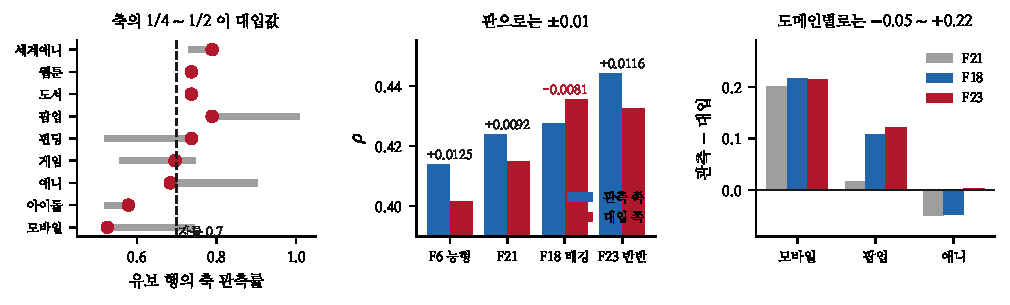
\includegraphics[width=\textwidth]{figs/imputed.pdf}
\caption{왼쪽 --- 축의 1/4$\sim$1/2 이 대입값. 가운데 --- 판으로는
$\pm$0.01. 오른쪽 --- 도메인별로는 $-$0.05$\sim$$+$0.22.}
\end{figure*}

\section{규모}

\begin{table}[t]
\centering\tsize
\caption{유보 행의 축 관측률(중앙 · 사분위).}
\begin{tabular}{lrrr}
\toprule
& 1분위 & 중앙 & 3분위 \\
\midrule
세계애니 & .737 & .789 & .789 \\
팝업 & .789 & .789 & 1.000 \\
웹툰 · 도서 & .737 & .737 & .737 \\
게임 & .565 & .696 & .739 \\
애니 & .684 & .684 & .895 \\
아이돌 & .526 & .579 & .579 \\
\textbf{모바일} & \textbf{.526} & \textbf{.526} & \textbf{.737} \\
\bottomrule
\end{tabular}
\end{table}

\claimx{\textbf{모든 행에서 축의 4분의 1에서 절반이 대입값이다.} 모바일은
중앙이 0.526 이라 절반 가까이가 채운 값이다.}{\textbf{웹툰 · 도서는
사분위가 전부 같다} --- 행마다 관측 무늬가 동일해서 이 검정이 아예 안
된다. \textbf{자를 수 있는 도메인이 애초에 전부가 아니다.}}

\section{판으로는 안 갈린다}

\begin{table}[t]
\centering\tsize
\caption{관측률 0.7 로 가른 두 판.}
\begin{tabular}{lrrrr}
\toprule
& 판 & 관측 & 대입 & 차 \\
\midrule
F6 능형 & .4250 & .4139 & .4014 & $+$.0125 \\
F21 & .4377 & .4239 & .4147 & $+$.0092 \\
\textbf{F18 배깅} & .4409 & .4274 & .4355 & \textbf{$-$.0081} \\
F23 반반 & .4524 & .4440 & .4324 & $+$.0116 \\
\midrule
\multicolumn{2}{l}{표본} & 1{,}653 & 871 & \\
\bottomrule
\end{tabular}
\end{table}

\claimx{\textbf{판 전체로는 $\pm$0.01 이다.} 여기서 멈추면 ``대입이
공짜도 아니고 벌도 아니다''가 된다.}{\textbf{그리고 계열이 갈린다} ---
선형 둘은 관측 쪽이 낫고 \textbf{트리는 대입 쪽이 낫다}($-$0.0081).
능형은 대입값을 계수에 그대로 넣고 트리는 관측 표시자를 갈라 쓰기
때문으로 읽히는데, \textbf{그것은 짐작이고 안 쟀다}(노트 232에서 기전
짐작을 세 번 틀렸다).}

\section{도메인별로는 크게 갈린다}

\begin{table}[t]
\centering\tsize
\caption{관측 $-$ 대입, 도메인별(자를 수 있는 셋).}
\begin{tabular}{lrrr}
\toprule
& F21 & F18 & F23 \\
\midrule
\textbf{모바일} & \textbf{$+$.201} & \textbf{$+$.217} & \textbf{$+$.215} \\
팝업 & $+$.017 & $+$.108 & $+$.122 \\
\textbf{애니} & \textbf{$-$.049} & \textbf{$-$.047} & $+$.002 \\
\bottomrule
\end{tabular}
\end{table}

\claimx{\textbf{모바일은 $+$0.21 이고 애니는 $-$0.05 다.} 판 $\pm$0.01 은
큰 값들이 서로 지운 결과다.}{모바일은 관측률 중앙이 0.526 으로 제일
낮다 --- \textbf{채운 것이 제일 많은 도메인에서 채운 행이 제일 안
맞는다.} 애니는 관측률이 0.684$\sim$0.895 로 높고 부호가 반대다.}

\claimx{\textbf{이 모양을 이 사이클에서 세 번째로 본다.} 노트 225(라벨
성질로 가르니 계열 순위가 뒤집혔다) · 노트 231(덮음으로 가르니 기준선이
죽어 있었다) · 이 노트(관측률).}{\textbf{판 $\rho$ 는 평균이고 평균은
반대 방향을 지운다.} 셋 다 ``하나의 수 뒤에 부호가 다른 것들이 있었다''
이고, 셋 다 \emph{가르기 전에는 안 보였다}.}

\claimx{\texttt{rank.by\_obs} 로 올려 \texttt{by\_kind} 옆에 나란히
적는다. \textbf{순위에는 안 쓴다} --- 판정치를 바꾸는 것이 아니라 셋으로
적는 것이다.}{노트 225가 렌즈 하나를 만들었고 이것이 둘째다.
\textbf{렌즈가 늘면 판 하나로 볼 때 안 보이던 것이 계속 나온다} ---
지금까지 셋 중 둘이 그 자리에서 값이 됐다(노트 227의 섞기, 노트 232의
고침).}

\begin{table}[t]
\centering\tsize
\caption{남은 것.}
\begin{tabular}{ll}
\toprule
\textbf{왜 트리는 반대인가} & 짐작만 있고 안 쟀다 \\
\textbf{모바일} & 관측률 0.526 --- 무엇이 비어 있나 \\
자를 수 없는 넷 & 웹툰 · 도서는 관측 무늬가 상수 \\
\bottomrule
\end{tabular}
\end{table}

둘째 줄이 값이 크고 곧바로 잴 수 있다. \textbf{모바일은 관측률 중앙이
0.526 으로 제일 낮고, 관측 $-$ 대입 격차도 $+$0.21 로 제일 크다} ---
판의 17.2\% 를 차지하는 도메인에서 절반 가까운 축이 채운 값이고 그
행들이 훨씬 안 맞는다. \textbf{무엇이 비어 있는지는 이미 안다} --- 노트
221이 모바일 검색 덮음을 54.2\% $\to$ 60.1\% 로 올렸고 아직 40\% 가
비어 있다. \textbf{노트 220의 천장표가 모바일 검색을 $+$0.0669 로 쟀는데,
이 노트는 그 천장이 왜 아직 안 닿았는지를 준다} --- 채운 행에서는 그
축이 아무것도 안 하기 때문이다.

\end{document}
